\chapter{The Machine Learning Landscape\label{The Machine Learning Landscape}}
Where does Machine Learning start and where does it end? What exactly does it
mean for a machine to learn something? If I download a copy of Wikipedia, has my
computer really learned something? Is it suddenly smarter? In this chapter we will
start by clarifying what Machine Learning is and why you may want to use it.

Then, before we set out to explore the Machine Learning continent, we will take a
look at the map and learn about the main regions and the most notable landmarks:
supervised versus unsupervised learning, online versus batch learning, instance-
based versus model-based learning. Then we will look at the workflow of a typical ML
project, discuss the main challenges you may face, and cover how to evaluate and
fine-tune a Machine Learning system.

This chapter introduces a lot of fundamental concepts (and jargon) that every data
scientist should know by heart. It will be a high-level overview (it’s the only chapter
without much code), all rather simple, but you should make sure everything is crystal
clear to you before continuing on to the rest of the book.

\textbf{Tips:} If you already know all the Machine Learning basics, you may want
to skip directly to \autoref{End-to-End Machine Learning Project} \nameref{End-to-End Machine Learning Project}.

\section{What Is Machine Learning?}
Machine Learning is the science (and art) of programming computers so they can
learn from data.

Here is a slightly more general definition:
\begin{quotation}
[Machine Learning is the] field of study that gives computers the ability to learn
without being explicitly programmed.
\begin{flushright}
---Arthur Samuel, 1959
\end{flushright}
\end{quotation}

And a more engineering-oriented one:
\begin{quotation}
A computer program is said to learn from experience E with respect to some task T
and some performance measure P, if its performance on T, as measured by P,
improves with experience E.
\begin{flushright}
---Tom Mitchell, 1997
\end{flushright}
\end{quotation}

Your spam filter is a Machine Learning program that, given examples of spam emails
(e.g., flagged by users) and examples of regular (nonspam, also called “ham”) emails,
can learn to flag spam. The examples that the system uses to learn are called the train‐
ing set. Each training example is called a training instance (or sample). In this case, the
task T is to flag spam for new emails, the experience E is the training data, and the
performance measure P needs to be defined; for example, you can use the ratio of
correctly classified emails. This particular performance measure is called accuracy,
and it is often used in classification tasks.

\section{Why Use Machine Learning?}

Machine Learning can help humans learn (\autoref{Machine Learning can help humans learn}). ML algorithms can be
inspected to see what they have learned (although for some algorithms this can be
tricky). For instance, once a spam filter has been trained on enough spam, it can
easily be inspected to reveal the list of words and combinations of words that it
believes are the best predictors of spam. Sometimes this will reveal unsuspected correlations or new trends, and thereby lead to a better understanding of the problem. Applying ML techniques to dig into large amounts of data can help discover patterns that were not immediately apparent. This is called data mining.
\begin{figure}
\centering
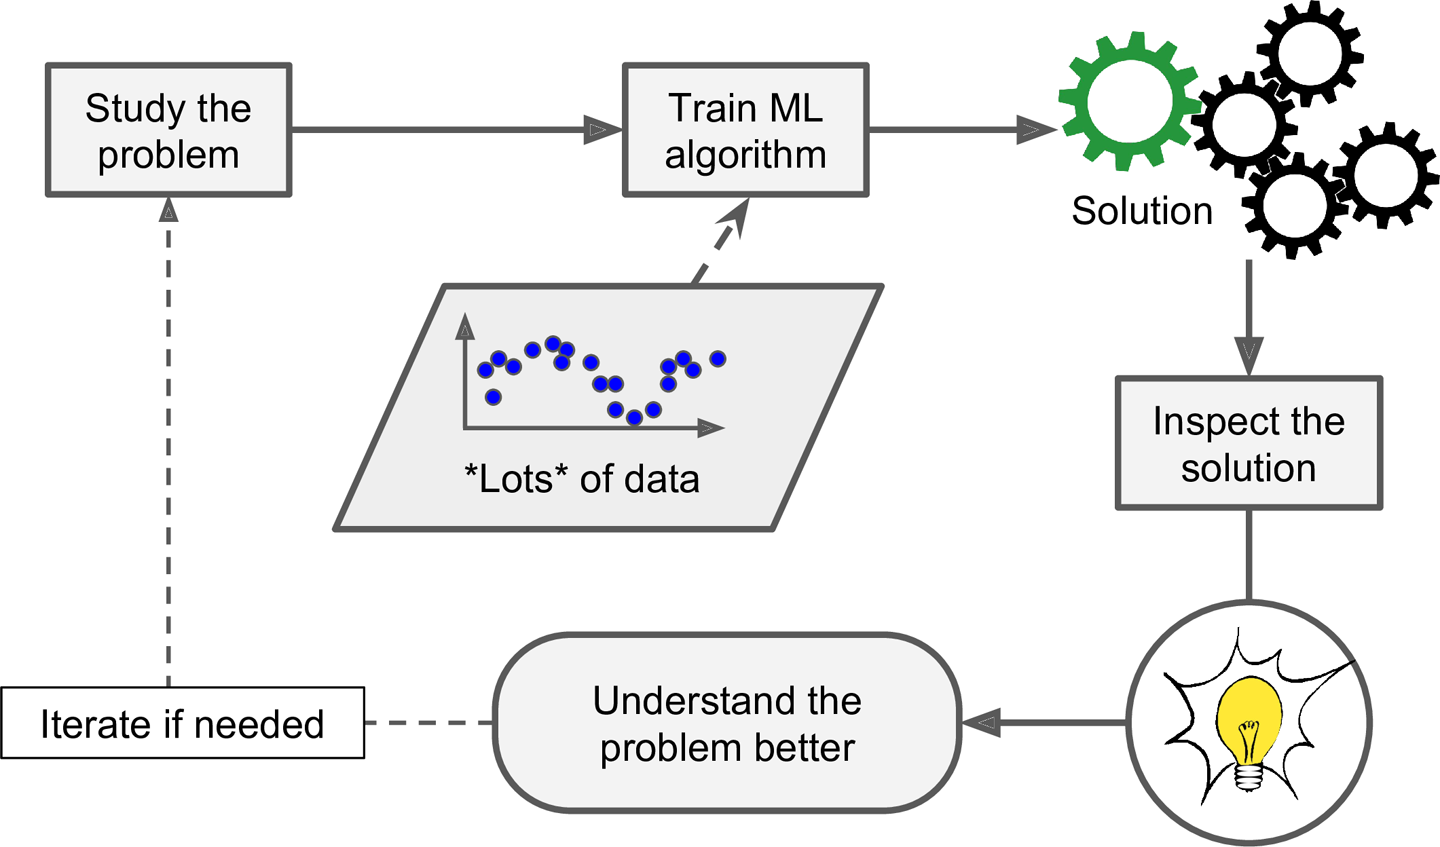
\includegraphics{img/Machine Learning can help humans learn.png}
\caption{Machine Learning can help humans learn}
\label{Machine Learning can help humans learn}
\end{figure}

To summarize, Machine Learning is great for:
\begin{itemize}
\item Problems for which existing solutions require a lot of fine-tuning or long lists of
rules: one Machine Learning algorithm can often simplify code and perform bet‐
ter than the traditional approach.
\item
 Complex problems for which using a traditional approach yields no good solu‐
tion: the best Machine Learning techniques can perhaps find a solution.
\item
 Fluctuating environments: a Machine Learning system can adapt to new data.
\item
 Getting insights about complex problems and large amounts of data.
\end{itemize}

\section{Examples of Applications}
\begin{itemize}
\item
\emph{Analyzing images of products on a production line to automatically classify them}

This is image classification, typically performed using convolutional neural net‐
works (CNNs; see \autoref{Deep Computer Vision Using
Convolutional Neural Networks}).
\item
\emph{Detecting tumors in brain scans}

This is semantic segmentation, where each pixel in the image is classified (as we
want to determine the exact location and shape of tumors), typically using CNNs
as well.
\item
\emph{Automatically classifying news articles}

This is natural language processing (NLP), and more specifically text classifica‐
tion, which can be tackled using recurrent neural networks (RNNs), CNNs, or
Transformers (see \autoref{Natural Language Processing with
RNNs and Attention}).
\item
\emph{Automatically flagging offensive comments on discussion forums}

This is also text classification, using the same NLP tools.
\item
\emph{Summarizing long documents automatically}

This is a branch of NLP called text summarization, again using the same tools.
\item
\emph{Creating a chatbot or a personal assistant}

This involves many NLP components, including natural language understanding
(NLU) and question-answering modules.
\item
\emph{Forecasting your company’s revenue next year, based on many performance metrics}

This is a regression task (i.e., predicting values) that may be tackled using any
regression model, such as a Linear Regression or Polynomial Regression model
(see \autoref{Training Models}), a regression SVM (see \autoref{Support Vector Machines}), a regression Random Forest
(see \autoref{Ensemble Learning and Random Forests}), or an artificial neural network (see \autoref{Introduction to Artificial Neural Networks
with Keras}). If you want to
take into account sequences of past performance metrics, you may want to use RNNs, CNNs, or Transformers (see Chapters \ref{Processing Sequences Using RNNs and CNNs} and \ref{Natural Language Processing with
RNNs and Attention}).
\item
\emph{Making your app react to voice commands}

This is speech recognition, which requires processing audio samples: since they
are long and complex sequences, they are typically processed using RNNs, CNNs,
or Transformers (see Chapters \ref{Processing Sequences Using
RNNs and CNNs} and \ref{Natural Language Processing with
RNNs and Attention}).
\item
\emph{Detecting credit card fraud}

This is anomaly detection (see \autoref{Unsupervised Learning Techniques}).
\item
\emph{Segmenting clients based on their purchases so that you can design a different marketing
strategy for each segment}

This is clustering (see \autoref{Unsupervised Learning Techniques}).
\item
\emph{Representing a complex, high-dimensional dataset in a clear and insightful diagram}

This is data visualization, often involving dimensionality reduction techniques
(see \autoref{Dimensionality Reduction}).
\item
\emph{Recommending a product that a client may be interested in, based on past purchases}

This is a recommender system. One approach is to feed past purchases (and
other information about the client) to an artificial neural network (see \autoref{Introduction to Artificial Neural Networks
with Keras}), and get it to output the most likely next purchase. This neural net would
typically be trained on past sequences of purchases across all clients.
\item
\emph{Building an intelligent bot for a game}

This is often tackled using Reinforcement Learning (RL; see \autoref{Reinforcement Learning}), which
is a branch of Machine Learning that trains agents (such as bots) to pick the
actions that will maximize their rewards over time (e.g., a bot may get a reward
every time the player loses some life points), within a given environment (such as
the game). The famous AlphaGo program that beat the world champion at the
game of Go was built using RL.
\end{itemize}

\section{Types of Machine Learning Systems}
There are so many different types of Machine Learning systems that it is useful to
classify them in broad categories, based on the following criteria:
\begin{itemize}
\item Whether or not they are trained with human supervision (supervised, unsupervised, semisupervised, and Reinforcement Learning)
\item Whether or not they can learn incrementally on the fly (online versus batch
learning)
\item Whether they work by simply comparing new data points to known data points,
or instead by detecting patterns in the training data and building a predictive
model, much like scientists do (instance-based versus model-based learning)
\end{itemize}

These criteria are not exclusive; you can combine them in any way you like. For
example, a state-of-the-art spam filter may learn on the fly using a deep neural network model trained using examples of spam and ham; this makes it an online, modelbased, supervised learning system.

\subsection{Supervised/Unsupervised Learning}
Machine Learning systems can be classified according to the amount and type of
supervision they get during training. There are four major categories: supervised
learning, unsupervised learning, semisupervised learning, and Reinforcement
Learning.

In supervised learning, the training set you feed to the algorithm includes the desired
solutions, called labels (\autoref{A labeled training set for spam classification}).
\begin{figure}
\centering
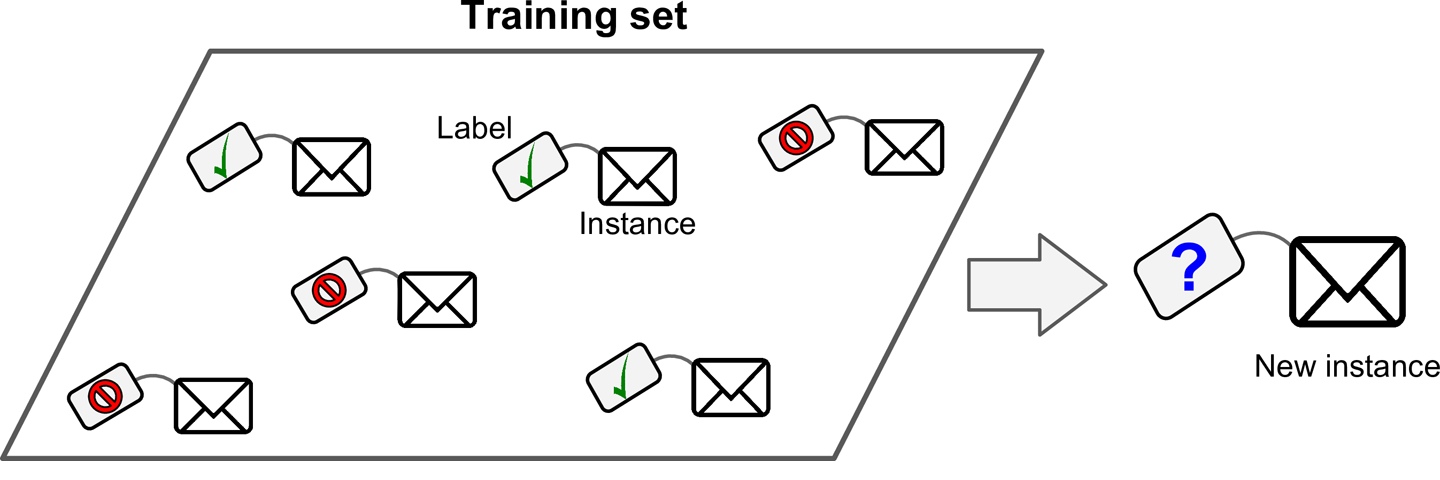
\includegraphics{img/A labeled training set for spam classification.png}
\caption{A labeled training set for spam classification}
\label{A labeled training set for spam classification}
\end{figure}

A typical supervised learning task is classification. The spam filter is a good example
of this: it is trained with many example emails along with their class (spam or ham),
and it must learn how to classify new emails.

Another typical task is to predict a target numeric value, such as the price of a car,
given a set of features (mileage, age, brand, etc.) called predictors. This sort of task is
called regression (\autoref{A regression problem predict a value, given an input feature})\footnote{Fun fact: this odd-sounding name is a statistics term introduced by Francis Galton while he was studying the
fact that the children of tall people tend to be shorter than their parents. Since the children were shorter, he
called this regression to the mean. This name was then applied to the methods he used to analyze correlations
between variables.}. To train the system, you need to give it many examples
of cars, including both their predictors and their labels (i.e., their prices).

\textbf{Notes:} In Machine Learning an attribute is a data type (e.g., “mileage”),
while a feature has several meanings, depending on the context, but
generally means an attribute plus its value (e.g., “mileage =
15,000”). Many people use the words attribute and feature interchangeably.

\begin{figure}
\centering
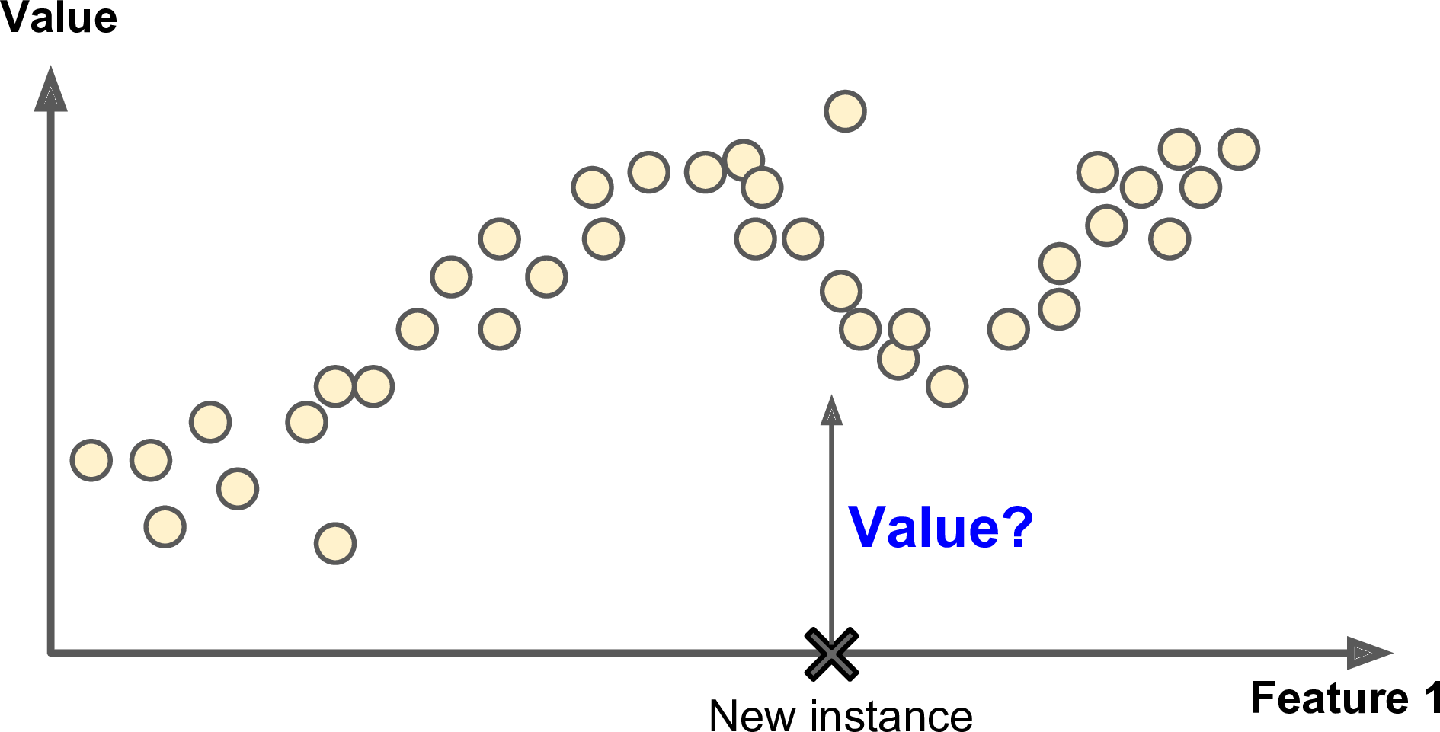
\includegraphics{img/A regression problem predict a value, given an input feature.png}
\caption{A regression problem: predict a value, given an input feature (there are usu‐
ally multiple input features, and sometimes multiple output values)}
\label{A regression problem predict a value, given an input feature}
\end{figure}

Here are some of the most important supervised learning algorithms (covered in this
book):
\begin{itemize}
\item
k-Nearest Neighbors
\item Linear Regression
\item Logistic Regression
\item Support Vector Machines (SVMs)
\item Decision Trees and Random Forests
\item Neural networks\footnote{Some neural network architectures can be unsupervised, such as autoencoders and restricted Boltzmann
machines. They can also be semisupervised, such as in deep belief networks and unsupervised pretraining}
\end{itemize}
\subsubsection{Unsupervised learning}
In unsupervised learning, as you might guess, the training data is unlabeled
(\autoref{An unlabeled training set for unsupervised learning}). The system tries to learn without a teacher.
\begin{figure}
\centering
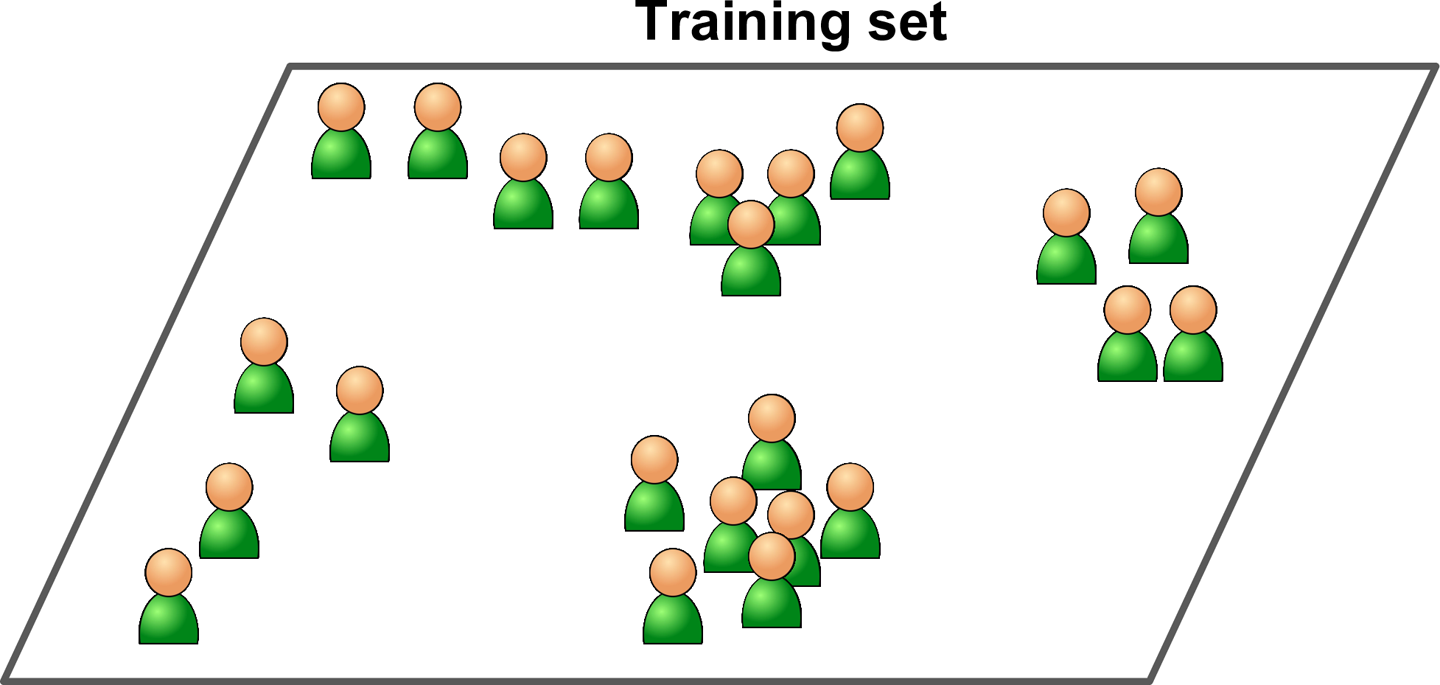
\includegraphics{img/An unlabeled training set for unsupervised learning.png}
\caption{An unlabeled training set for unsupervised learning}
\label{An unlabeled training set for unsupervised learning}
\end{figure}
Here are some of the most important unsupervised learning algorithms (most of
these are covered in Chapters \ref{Dimensionality Reduction} and \ref{Unsupervised Learning Techniques}):
\begin{itemize}
\item Clustering
\begin{itemize}
\item K-Means
\item DBSCAN
\item Hierarchical Cluster Analysis (HCA)
\end{itemize}
\item Anomaly detection and novelty detection
\begin{itemize}
\item One-class SVM
\item Isolation Forest
\end{itemize}

\item Visualization and dimensionality reduction
\begin{itemize}
\item Principal Component Analysis (PCA)
\item Kernel PCA
\item Locally Linear Embedding (LLE)
\item t-Distributed Stochastic Neighbor Embedding (t-SNE)
\end{itemize}
\item
 Association rule learning
\begin{itemize}
\item Apriori
\item Eclat
\end{itemize}
\end{itemize}

For example, say you have a lot of data about your blog’s visitors. You may want to
run a clustering algorithm to try to detect groups of similar visitors (\autoref{Clustering}). At
no point do you tell the algorithm which group a visitor belongs to: it finds those
connections without your help.
\begin{figure}
\centering
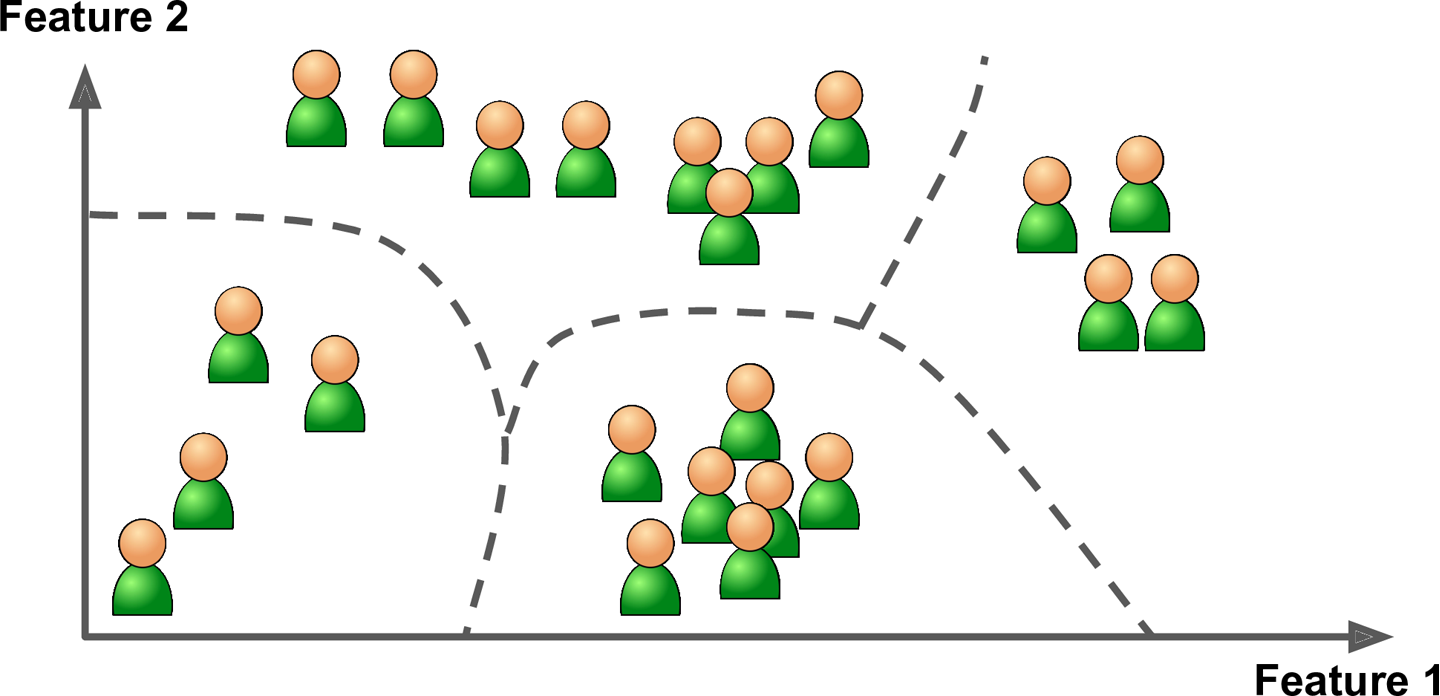
\includegraphics{img/Clustering.png}
\caption{Clustering}
\label{Clustering}
\end{figure}

Visualization algorithms are also good examples of unsupervised learning algorithms:
you feed them a lot of complex and unlabeled data, and they output a 2D or 3D rep‐
resentation of your data that can easily be plotted (\autoref{Example of a t-SNE visualization highlighting semantic clusters}\footnote{Notice how animals are rather well separated from vehicles and how horses are close to deer but far from
birds. Figure reproduced with permission from Richard Socher et al., “Zero-Shot Learning Through CrossModal Transfer,” Proceedings of the 26th International Conference on Neural Information Processing Systems 1
(2013): 935–943.}). These algorithms try
to preserve as much structure as they can (e.g., trying to keep separate clusters in the
input space from overlapping in the visualization) so that you can understand how
the data is organized and perhaps identify unsuspected patterns.
\begin{figure}
\centering
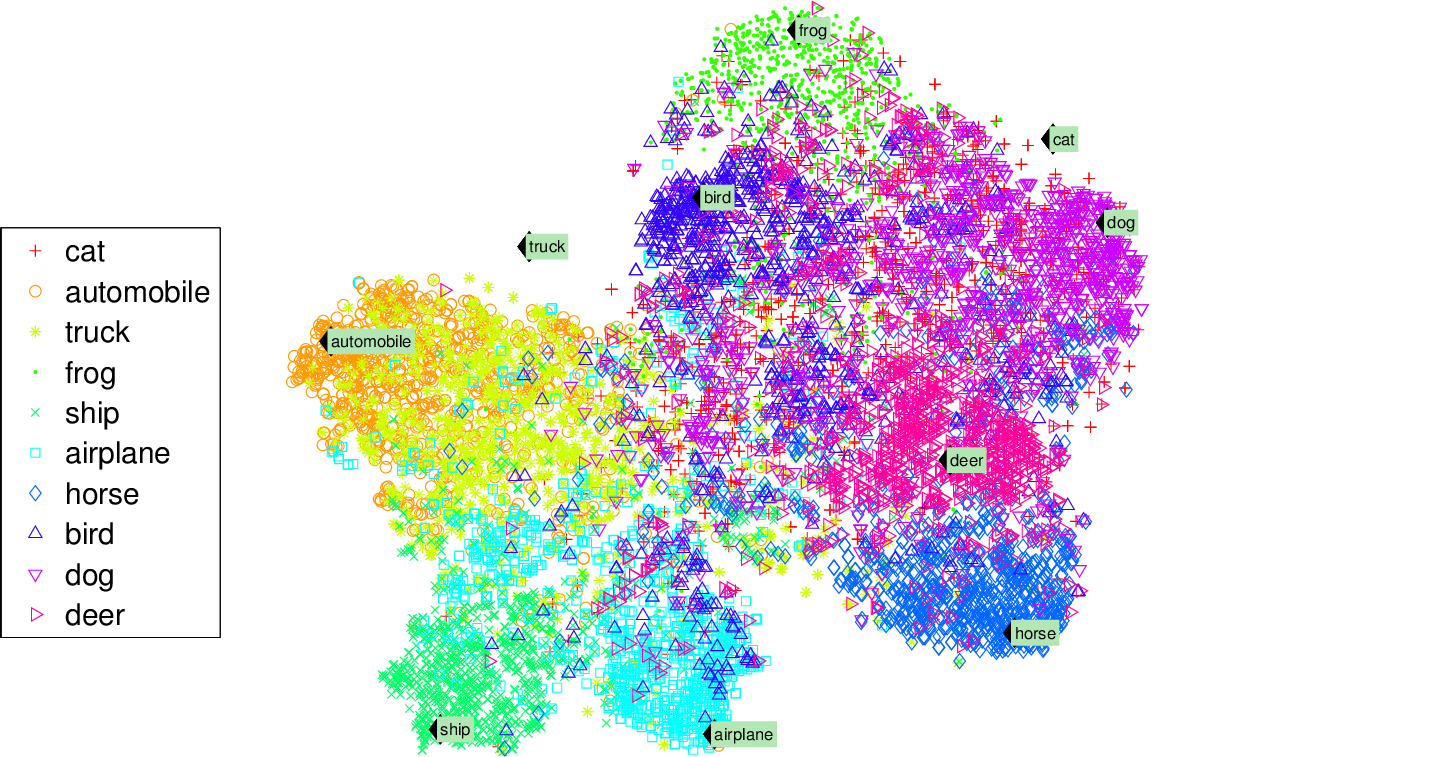
\includegraphics{img/Example of a t-SNE visualization highlighting semantic clusters.png}
\caption{Example of a t-SNE visualization highlighting semantic clusters}
\label{Example of a t-SNE visualization highlighting semantic clusters}
\end{figure}

A related task is dimensionality reduction, in which the goal is to simplify the data
without losing too much information. One way to do this is to merge several correla‐
ted features into one. For example, a car’s mileage may be strongly correlated with its
age, so the dimensionality reduction algorithm will merge them into one feature that
represents the car’s wear and tear. This is called feature extraction.

\textbf{Notes:} It is often a good idea to try to reduce the dimension of your train‐
ing data using a dimensionality reduction algorithm before you
feed it to another Machine Learning algorithm (such as a super‐
vised learning algorithm). It will run much faster, the data will take
up less disk and memory space, and in some cases it may also per‐
form better.

Yet another important unsupervised task is anomaly detection—for example, detect‐
ing unusual credit card transactions to prevent fraud, catching manufacturing defects,
or automatically removing outliers from a dataset before feeding it to another learn‐
ing algorithm. The system is shown mostly normal instances during training, so it
learns to recognize them; then, when it sees a new instance, it can tell whether it looks
like a normal one or whether it is likely an anomaly (see \autoref{Anomaly detection}). A very similar
task is novelty detection: it aims to detect new instances that look different from all
instances in the training set. This requires having a very “clean” training set, devoid of
any instance that you would like the algorithm to detect. For example, if you have
thousands of pictures of dogs, and 1\% of these pictures represent Chihuahuas, then a
novelty detection algorithm should not treat new pictures of Chihuahuas as novelties.
On the other hand, anomaly detection algorithms may consider these dogs as so rare
and so different from other dogs that they would likely classify them as anomalies (no
offense to Chihuahuas).
\begin{figure}
\centering
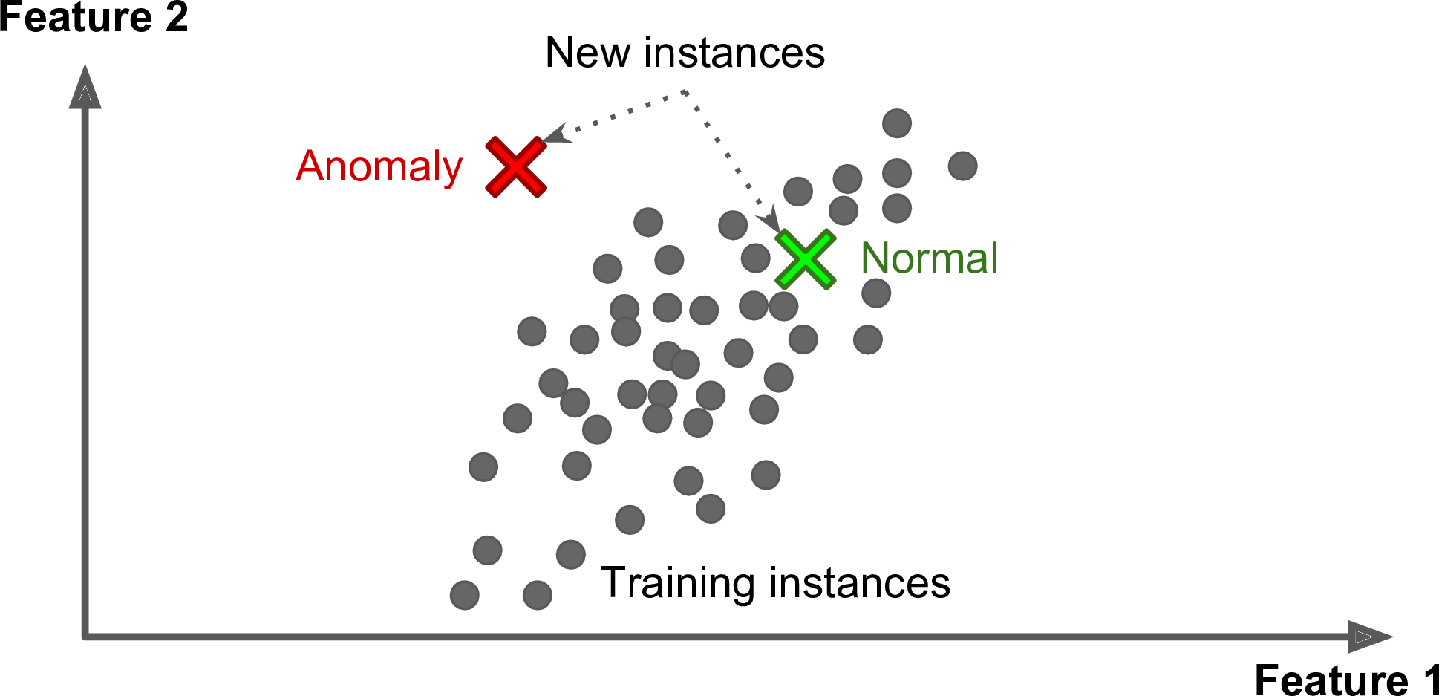
\includegraphics{img/Anomaly detection.png}
\caption{Anomaly detection}
\label{Anomaly detection}
\end{figure}

Finally, another common unsupervised task is association rule learning, in which the
goal is to dig into large amounts of data and discover interesting relations between attributes. For example, suppose you own a supermarket. Running an association rule
on your sales logs may reveal that people who purchase barbecue sauce and potato
chips also tend to buy steak. Thus, you may want to place these items close to one
another.

\subsubsection{Semisupervised learning}
Since labeling data is usually time-consuming and costly, you will often have plenty of
unlabeled instances, and few labeled instances. Some algorithms can deal with data
that’s partially labeled. This is called semisupervised learning (\autoref{Semisupervised learning with two classes}).

\begin{figure}
\centering
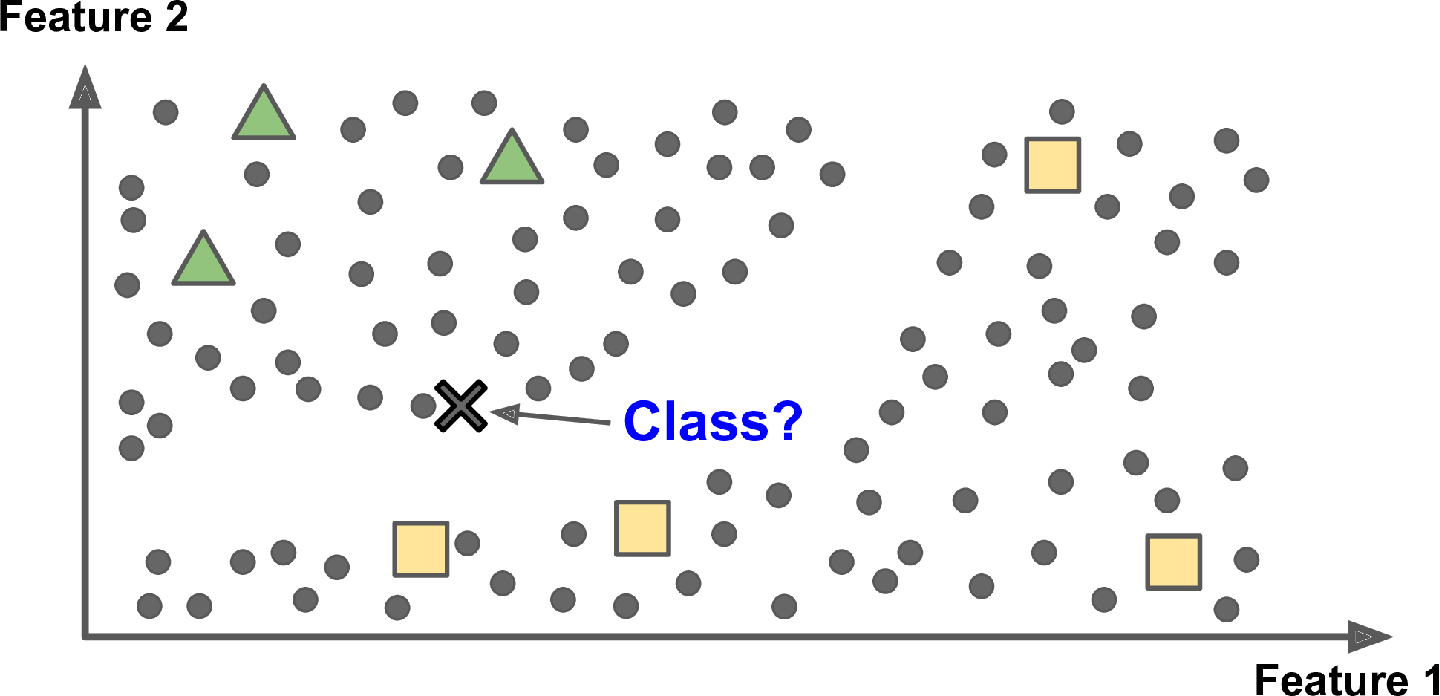
\includegraphics{img/Semisupervised learning with two classes.png}
\caption{Semisupervised learning with two classes (triangles and squares): the unlabeled examples (circles) help classify a new instance (the cross) into the triangle class
rather than the square class, even though it is closer to the labeled squares}
\label{Semisupervised learning with two classes}
\end{figure}

Most semisupervised learning algorithms are combinations of unsupervised and
supervised algorithms. For example, deep belief networks (DBNs) are based on unsu‐
pervised components called restricted Boltzmann machines (RBMs) stacked on top of
one another. RBMs are trained sequentially in an unsupervised manner, and then the
whole system is fine-tuned using supervised learning techniques.

\subsubsection{Reinforcement Learning}
Reinforcement Learning is a very different beast. The learning system, called an agent
in this context, can observe the environment, select and perform actions, and get
rewards in return (or penalties in the form of negative rewards, as shown in
\autoref{Reinforcement Learning}).
\begin{figure}
\centering
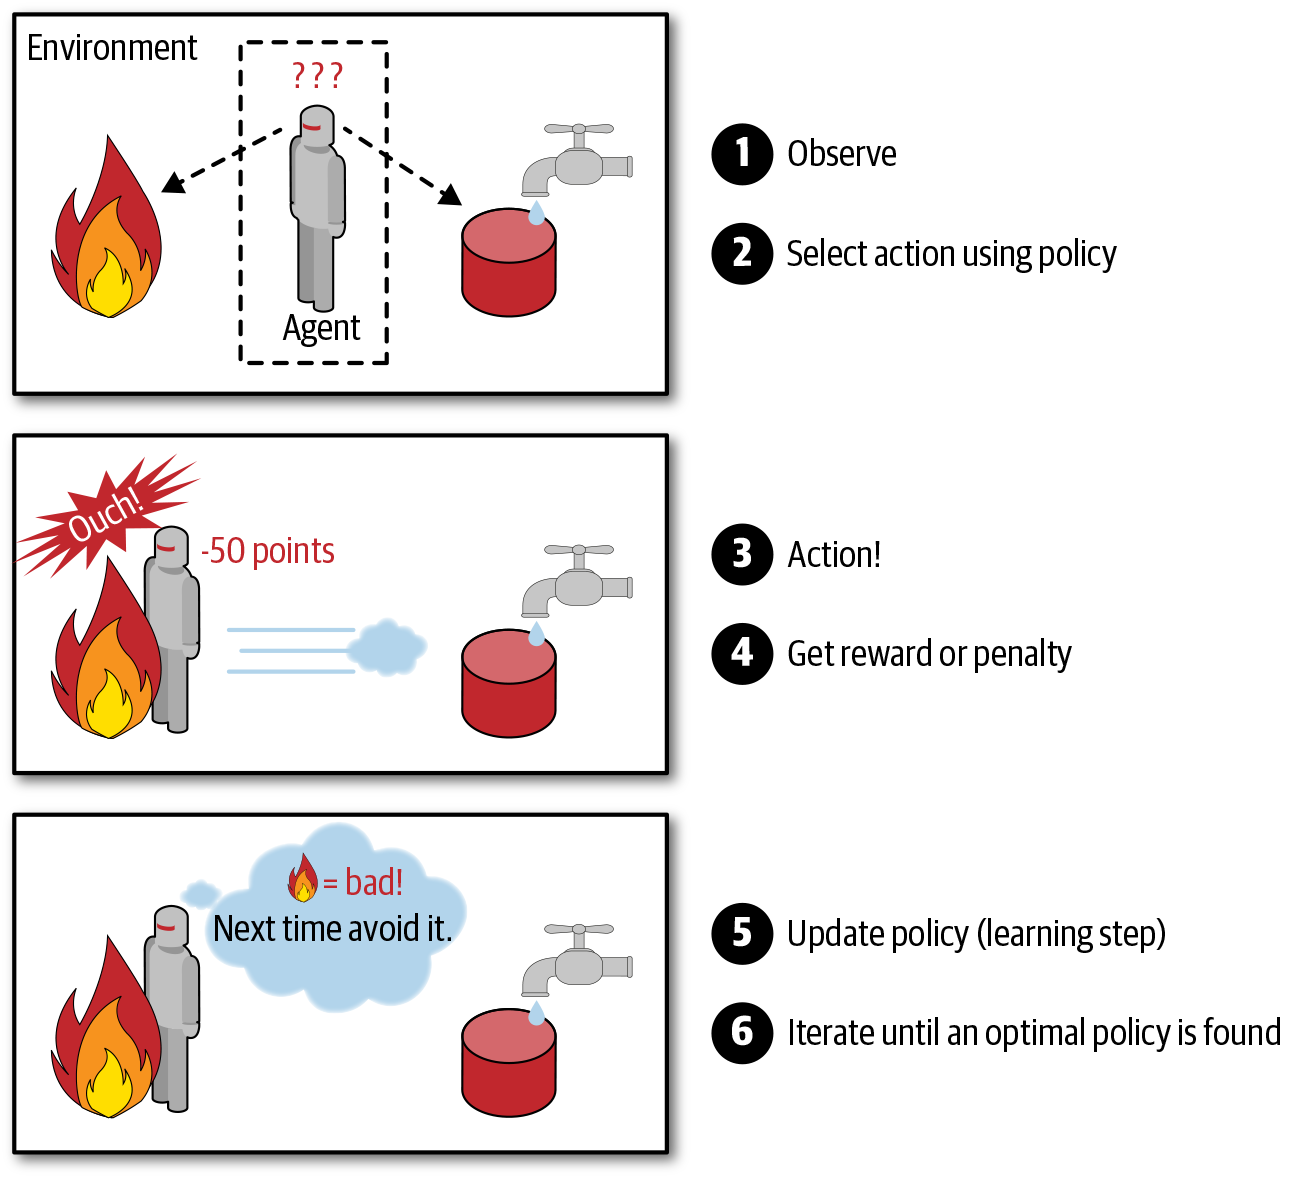
\includegraphics{img/Reinforcement Learning.png}
\caption{Reinforcement Learning}
\label{Reinforcement Learning}
\end{figure}
For example, many robots implement Reinforcement Learning algorithms to learn
how to walk. DeepMind’s AlphaGo program is also a good example of Reinforcement
Learning: it made the headlines in May 2017 when it beat the world champion Ke Jie
at the game of Go. It learned its winning policy by analyzing millions of games, and
then playing many games against itself. Note that learning was turned off during the
games against the champion; AlphaGo was just applying the policy it had learned.
\subsection{Batch and Online Learning}
Another criterion used to classify Machine Learning systems is whether or not the
system can learn incrementally from a stream of incoming data.

\subsubsection{Batch learning}
In batch learning, the system is incapable of learning incrementally: it must be trained
using all the available data. This will generally take a lot of time and computing
resources, so it is typically done offline. First the system is trained, and then it is
launched into production and runs without learning anymore; it just applies what it
has learned. This is called offline learning.

Training on the full set of data requires a lot of computing resources (CPU,
memory space, disk space, disk I/O, network I/O, etc.). If you have a lot of data and
you automate your system to train from scratch every day, it will end up costing you a
lot of money. If the amount of data is huge, it may even be impossible to use a batch
learning algorithm.

\subsubsection{Online learning}
In online learning, you train the system incrementally by feeding it data instances
sequentially, either individually or in small groups called mini-batches. Each learning
step is fast and cheap, so the system can learn about new data on the fly, as it arrives
(see \autoref{In online learning}).
\begin{figure}
\centering
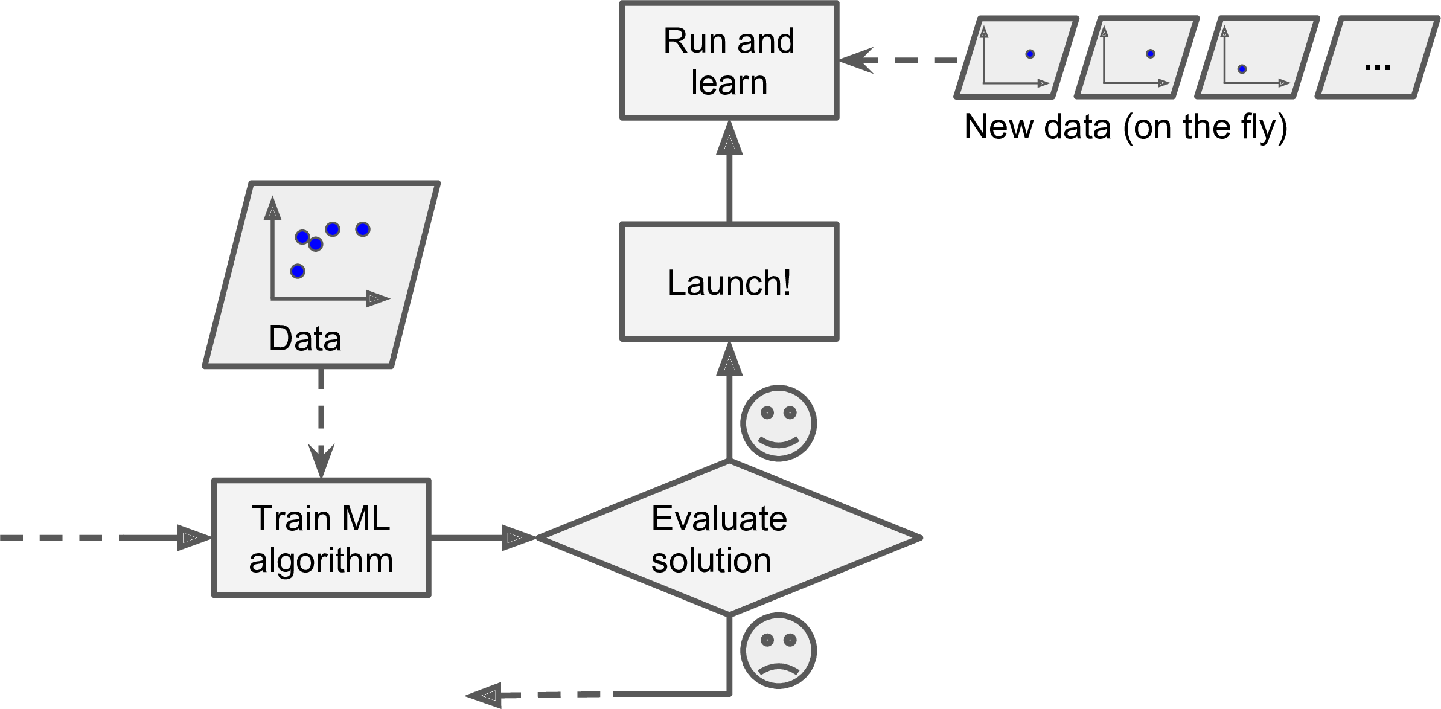
\includegraphics{img/online learning.png}
\caption{In online learning, a model is trained and launched into production, and
then it keeps learning as new data comes in}
\label{In online learning}
\end{figure}

Online learning is great for systems that receive data as a continuous flow (e.g., stock
prices) and need to adapt to change rapidly or autonomously. It is also a good option
if you have limited computing resources: once an online learning system has learned
about new data instances, it does not need them anymore, so you can discard them
(unless you want to be able to roll back to a previous state and “replay” the data). This
can save a huge amount of space.

Online learning algorithms can also be used to train systems on huge datasets that
cannot fit in one machine’s main memory (this is called out-of-core learning). The
algorithm loads part of the data, runs a training step on that data, and repeats the
process until it has run on all of the data (see \autoref{Using online learning to handle huge datasets}).
\begin{figure}
\centering
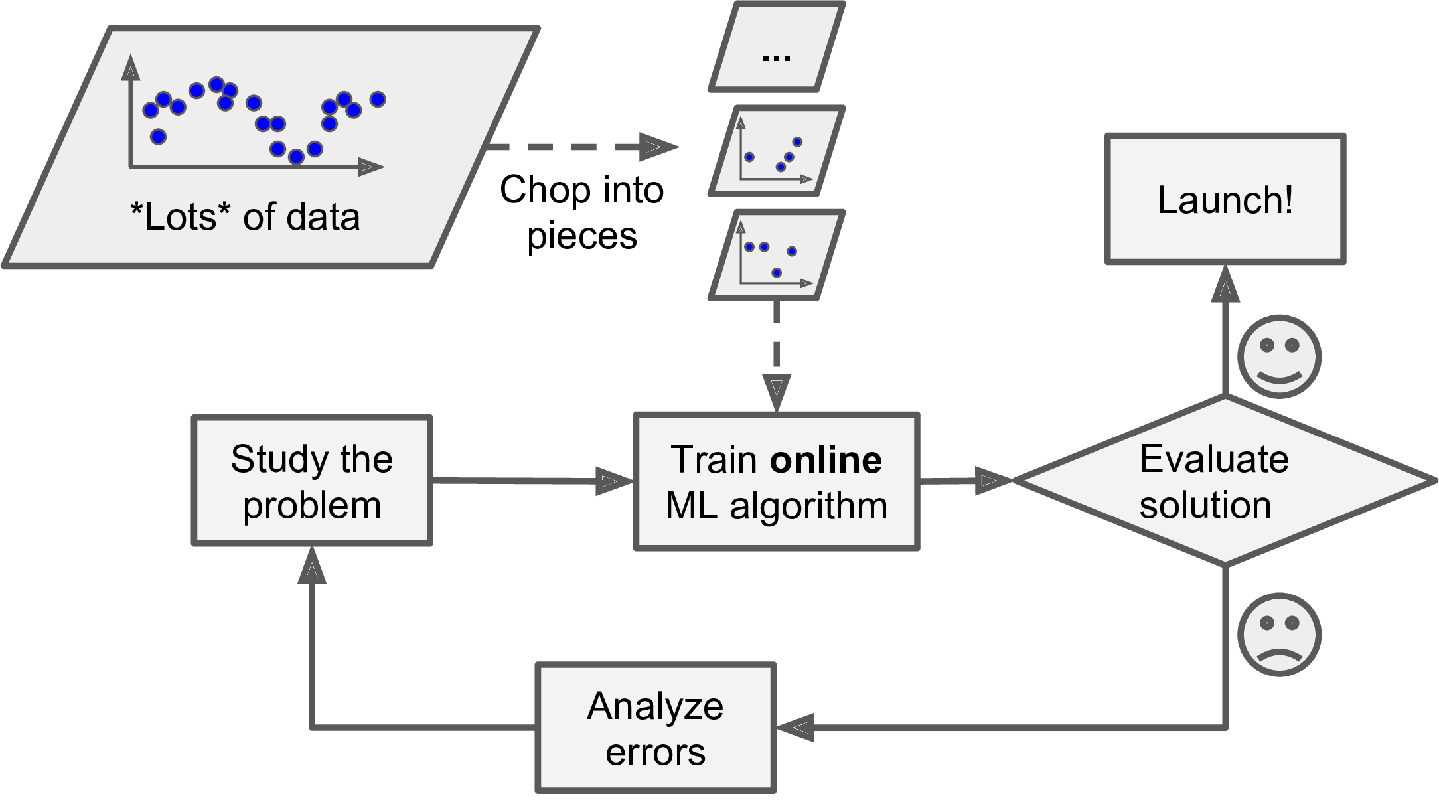
\includegraphics{img/Using online learning to handle huge datasets.png}
\caption{Using online learning to handle huge datasets}
\label{Using online learning to handle huge datasets}
\end{figure}

\textbf{Cautions:} Out-of-core learning is usually done offline (i.e., not on the live
system), so online learning can be a confusing name. Think of it as
incremental learning.

A big challenge with online learning is that if bad data is fed to the system, the system’s performance will gradually decline. If it’s a live system, your clients will notice.
For example, bad data could come from a malfunctioning sensor on a robot, or from
someone spamming a search engine to try to rank high in search results. To reduce
this risk, you need to monitor your system closely and promptly switch learning off
(and possibly revert to a previously working state) if you detect a drop in performance. You may also want to monitor the input data and react to abnormal data (e.g.,
using an anomaly detection algorithm).
\subsection{Instance-Based Versus Model-Based Learning}
One more way to categorize Machine Learning systems is by how they generalize.
Most Machine Learning tasks are about making predictions. This means that given a
number of training examples, the system needs to be able to make good predictions
for (generalize to) examples it has never seen before. Having a good performance
measure on the training data is good, but insufficient; the true goal is to perform well
on new instances.

There are two main approaches to generalization: instance-based learning and
model-based learning.

\subsubsection{Instance-based learning}
Possibly the most trivial form of learning is simply to learn by heart. If you were to
create a spam filter this way, it would just flag all emails that are identical to emails
that have already been flagged by users—not the worst solution, but certainly not the
best.

Instead of just flagging emails that are identical to known spam emails, your spam
filter could be programmed to also flag emails that are very similar to known spam
emails. This requires a \emph{measure of similarity} between two emails. A (very basic) similarity measure between two emails could be to count the number of words they have
in common. The system would flag an email as spam if it has many words in common with a known spam email.

This is called \emph{instance-based learning}: the system learns the examples by heart, then
generalizes to new cases by using a similarity measure to compare them to the
learned examples (or a subset of them). For example, in \autoref{Instance-based learning} the new instance
would be classified as a triangle because the majority of the most similar instances
belong to that class.
\begin{figure}
\centering
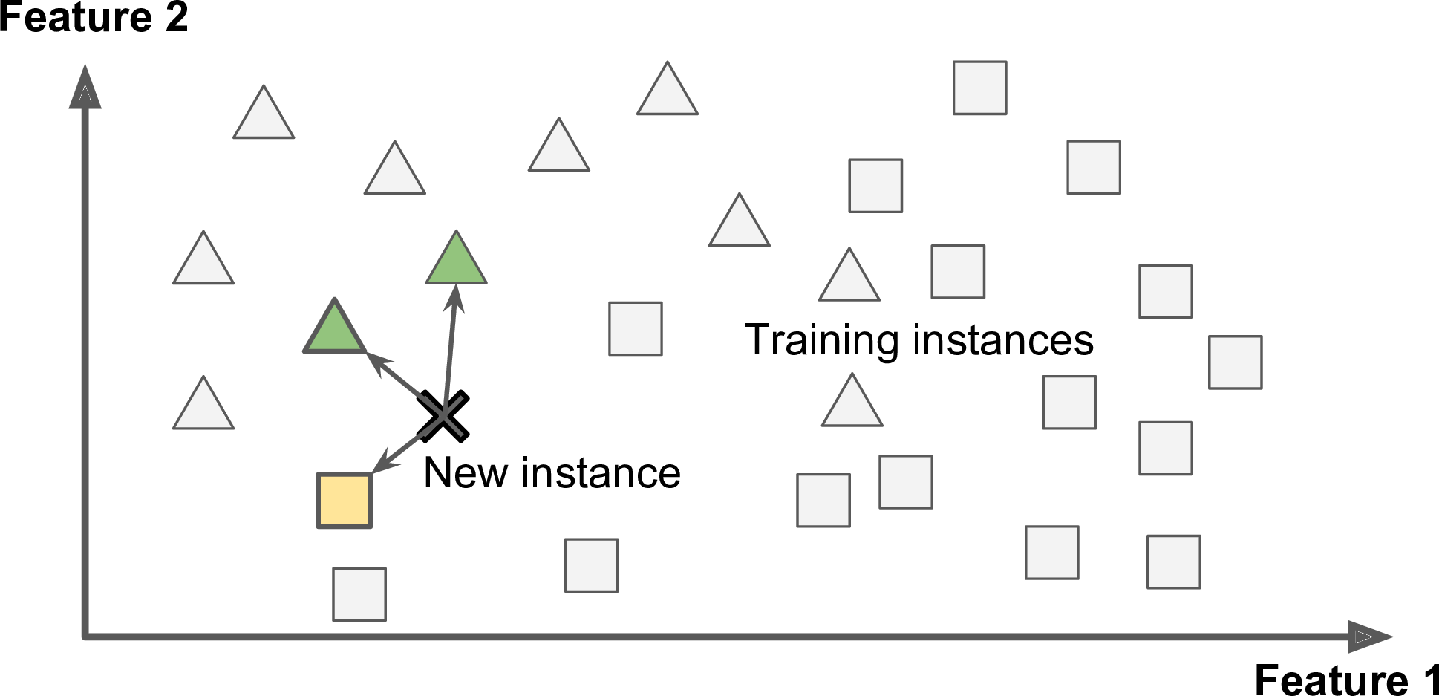
\includegraphics{img/Instance-based learning.png}
\caption{Instance-based learning}
\label{Instance-based learning}
\end{figure}

\subsubsection{Model-based learning}
Another way to generalize from a set of examples is to build a model of these exam‐
ples and then use that model to make predictions. This is called model-based learning
(\autoref{Model-based learning}).
\begin{figure}
\centering
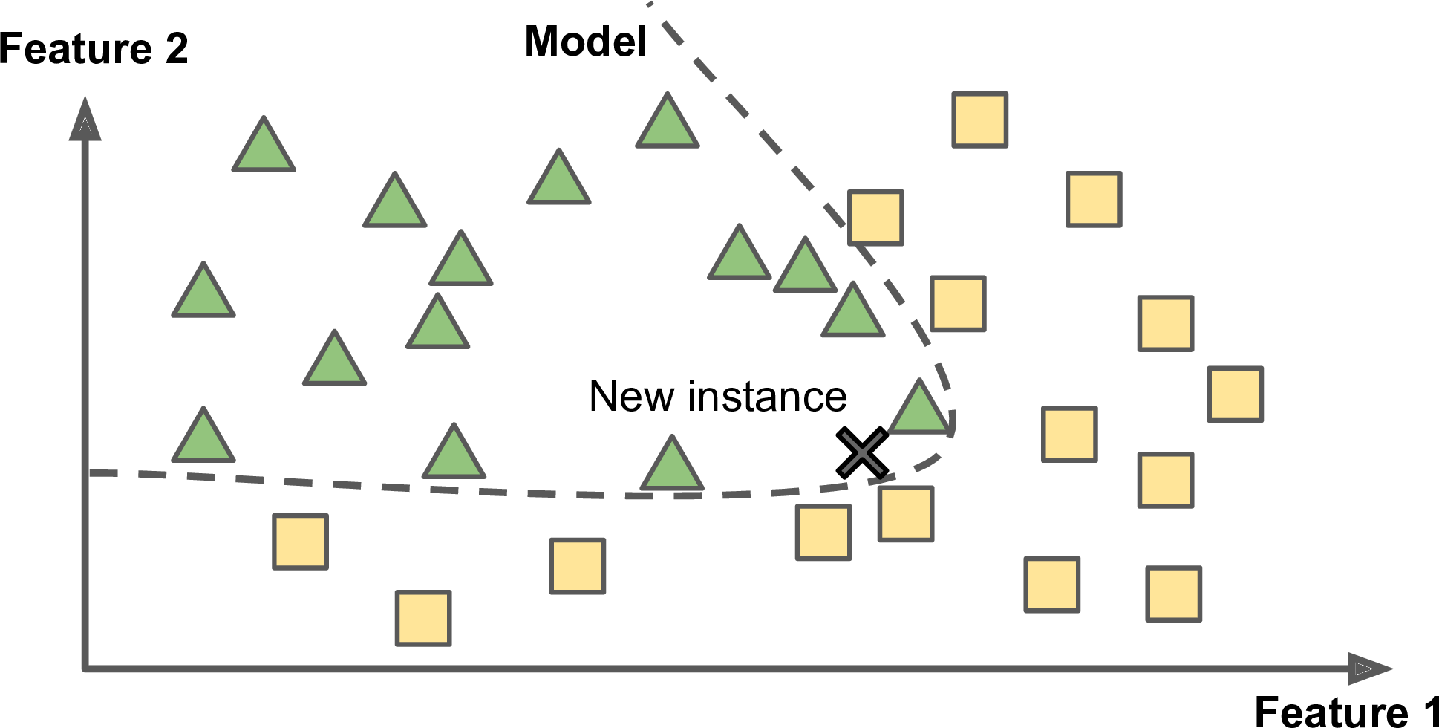
\includegraphics{img/Model-based learning.png}
\caption{Model-based learning}
\label{Model-based learning}
\end{figure}

For example, suppose you want to know if money makes people happy, so you download the Better Life Index data from the \href{https://stats.oecd.org/index.aspx?DataSetCode=BLI}{OECD’s website} and stats about gross domestic product (GDP) per capita from the \href{https://www.imf.org/en/Publications/SPROLLS/world-economic-outlook-databases#sort=\%40imfdate\%20descending}{IMF’s website}.
